
\chapter{Required software}
\section{The overview of required software}

Building a DNS server for TRR needs some software, including the software for implementing DNS server, operation system, tools and server \cite{DNS_resources}.
\\

The DNS server need tools to recieve DoH queries and test. DoH-proxy is designed for this purpose, the developer is Facebook. It can be installed on Linux but it requires Python 3.5 \cite{doh_proxy}.
\\

After that, NGINX can provide the web service. NGINX is a HTTP server with high performance, it can also provide different kinds of services. The operator can set the method for listening queries in a port and the request from users \cite{NGINX_wiki}.
\\

About Operating System, Linux is recommended, because the much resource for building DNS servers is based on Linux \cite{configure_BIND}.
\\

The required software is shown in TABLE ~\ref{tab:required_software}.
\\

\begin{table}[hbt!]
    \centering
    \begin{tabular}{|c|c|c|}
        \hline
         Category & Software & Note\\    
        \hline
         DNS & BIND 9 & \\
        \hline
         DNS & Unbound & Free and open-source software\\
        \hline
         DNS & PowerDNS & \\
        \hline
         Tool & DoH-proxy &  \\
        \hline
        Server & NGINX & Free and open-source software\\
        \hline
    \end{tabular}
    \caption{The required software for building a DNS server for TRR}
    \label{tab:required_software}
\end{table}

\section{Comparison of DNS software}

There are many choices to implement a DNS server, such as BIND, Unbound, DNSMASQ, PowerDNS, Microsoft DNS and Cisco Network Registrar \cite{DNS_software_wiki} \cite{Bind_dnsmasq_PowerDNS_Unbound}. In this research, Unbound, BIND and PowerDNS are recommended, because there are many discussion about those three software on Internet, moreover, they support DNS over HTTPS (DoH), then users may use TRR to browse websites in Firefox \cite{Building_DOH} \cite{DNS_over_HTTPS_servers}.
\\

Unbound is the free open-source software which focuses on building a recursive DNS server, it does not support the authoritative DNS server. The developer is NLnet Labs, the developer also designed another DNS software, which is NSD(Name Server Daemon), in contrast, NSD is only for building authoritative DNS servers \cite{NSD_wiki}. Unbound supports some security functions, such as Domain Name System Security Extensions(DNSSEC) and DNS over TLS(DoT). Moreover, the operating systems for running Unbound can be Linux, FreeBSD and Windows \cite{Unbound_wiki}.
\\

About BIND, its alias is Named. Unlike Unbound, it supports both recursive and authoritative DNS servers. It is developed by Internet Systems Consortium(ISC). ISC is also the organization which is responsible for managing F root server zone. The stable version is BIND 9. It can run on Windows, Mac-OS and Linux \cite{BIND_wiki}.
\\

PowerDNS, it supports both authoritative DNS server and recursive DNS server, moreover, it provides a Graphic UI for management and uses relational databases to store data. The developer is PowerDNS Community and operating systems are Linux and FreeBSD  \cite{PowerDNS_wiki}.
\\

Compare with Unbound, BIND and PowerDNS, those three software are all good choices \cite{Compare_the_different_DNS_servers}.
\\

For the consideration about the performance, there are some difference among BIND, Unbound and PowerDNS.
\\

According to a report which was written by Hamza Boulakhrif in University of Amsterdam, The times for processing queries in BIND, Unbound and PowerDNS were similar. The biggest difference was that when the time of processing exceeded 16 seconds, then PowerDNS did not response. If the time exceeded 17 seconds, BIND did not response, only Unbound can wait until the finish of processing then sent results to users \cite{DNS_resolver_performance_measurements}.
\\

The processing time in those 3 DNS software in this report is shown in Fig.~\ref{fig:DNS_resolver_performance_measurements}.
\\

\begin{figure}[hbt!]  
    \centering
    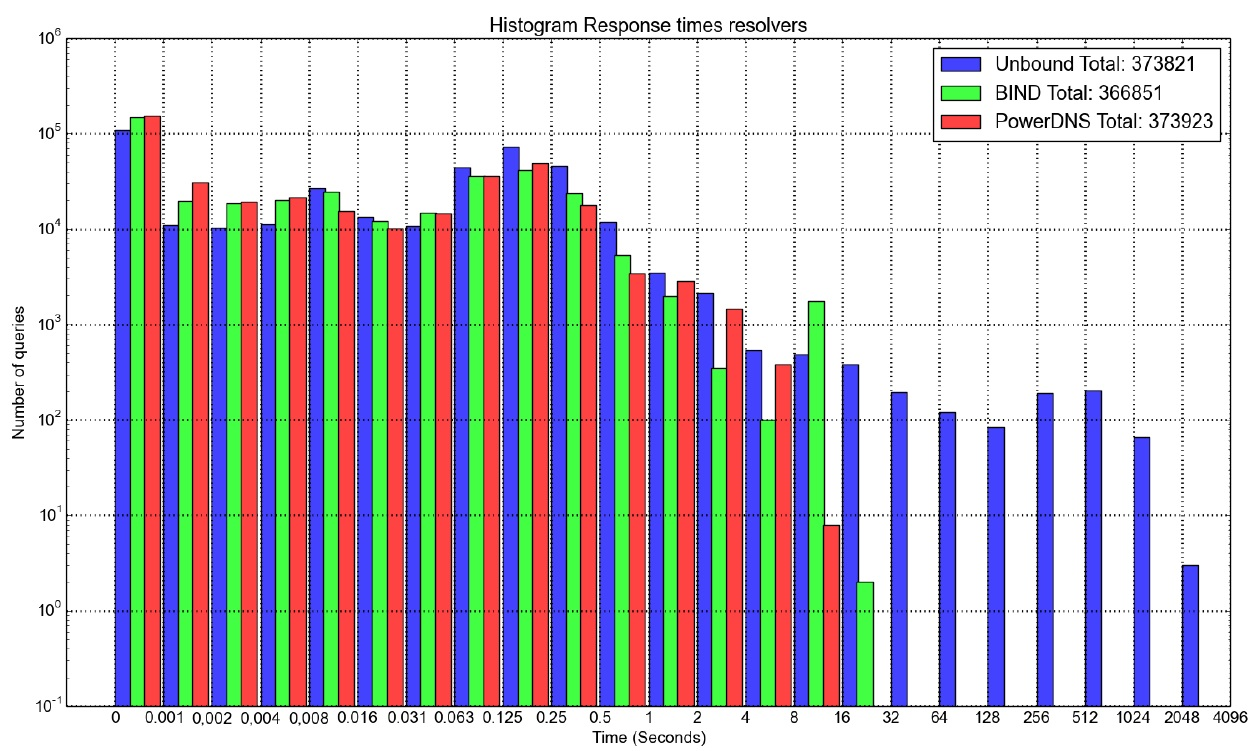
\includegraphics[width=0.8\textwidth]{figure/DNS-resolver-measurement.jpg}
    \caption{\em The processing time in BIND, Unbound and PowerDNS \cite{DNS_resolver_performance_measurements} \label{fig:DNS_resolver_performance_measurements}}
\end{figure}


In Fig.~\ref{fig:DNS_resolver_performance_measurements}, according to the assumption of Hamza Boulakhrif, if processing time is under 1 milliseconds, then it is processed by the cache, because the caches in DNS servers contain the matched IP addresses that users are looking for, thus DNS servers can response users in a very short time and do not need to ask authoritative DNS servers.
\\

\begin{figure}[hbt!]  
    \centering
    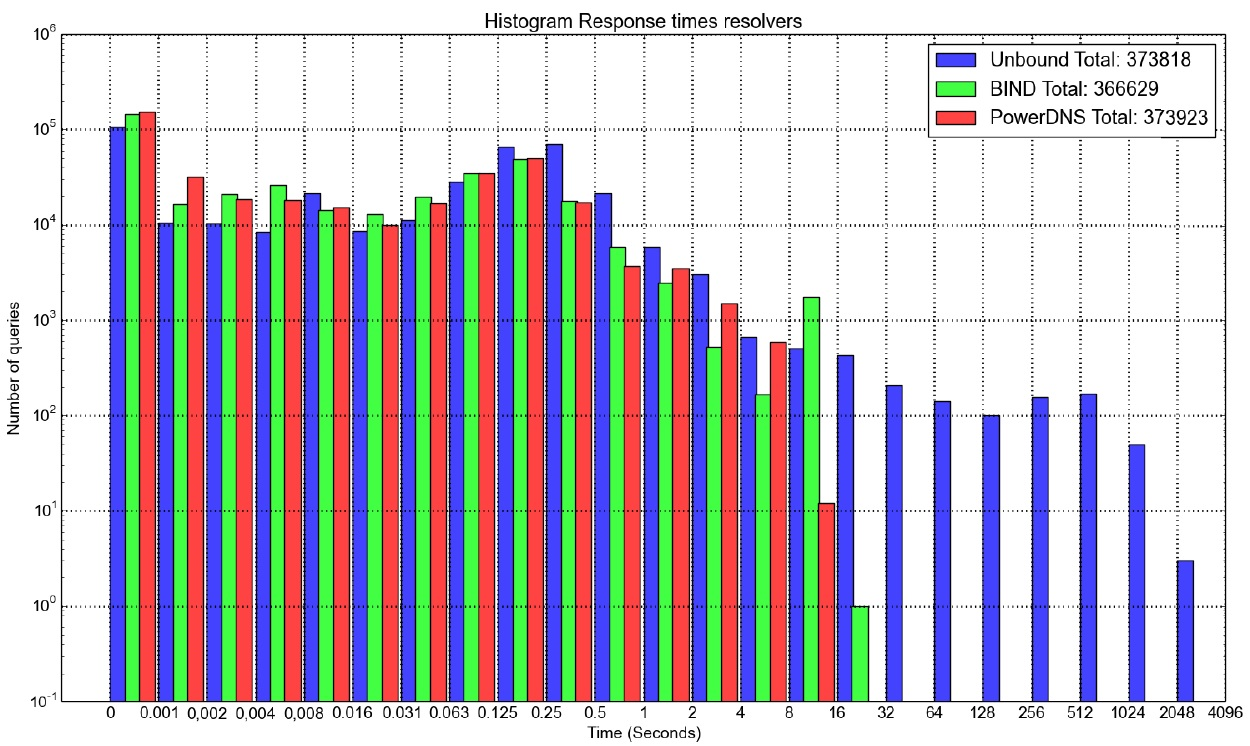
\includegraphics[width=0.8\textwidth]{figure/DNS-resolver-measurement-DNSSEC.jpg}
    \caption{\em The processing time in BIND, Unbound and PowerDNS with DNSSEC \cite{DNS_resolver_performance_measurements} \label{fig:DNS_resolver_performance_measurements_DNSSEC}}
\end{figure}


In the other experiment, BIND, Unbound and PowerDNS ran with DNSSEC, there was no obvious change if compare it with these DNS servers without DNSSEC. The result of using DNSSEC is shown in Fig.~\ref{fig:DNS_resolver_performance_measurements_DNSSEC}.
\\

\begin{figure}[hbt!]  
    \centering
    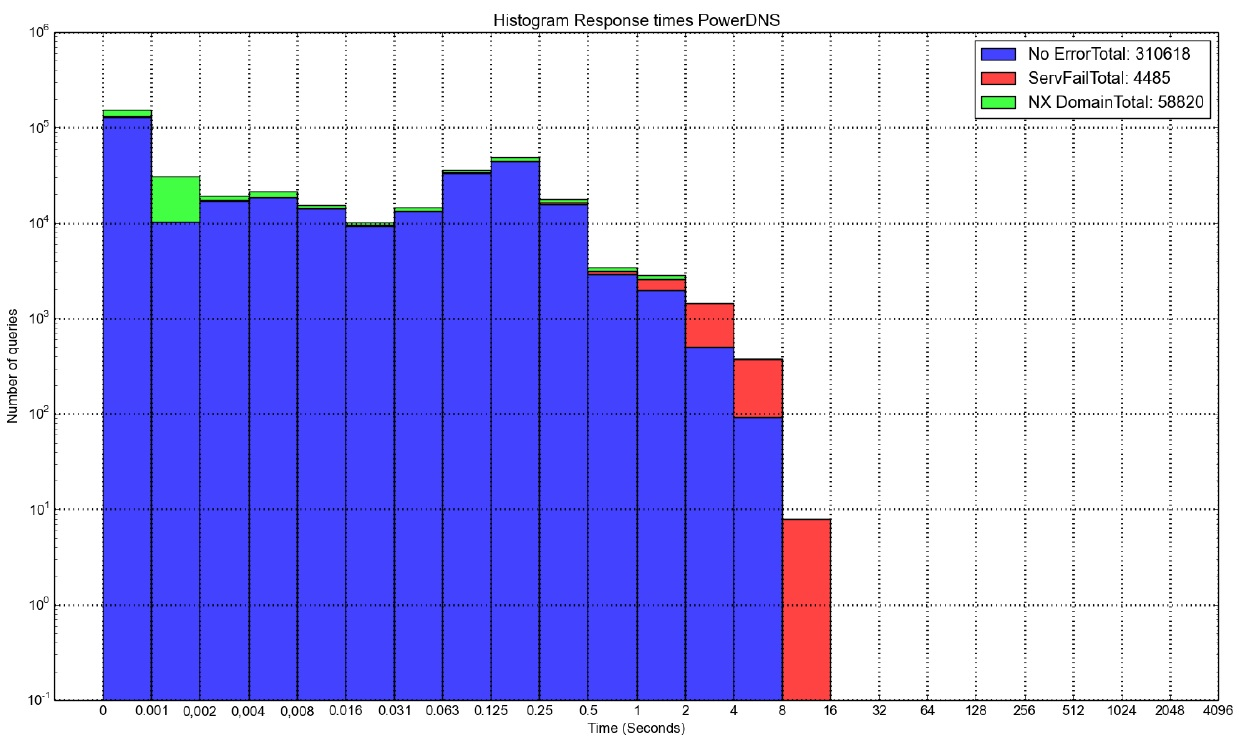
\includegraphics[width=0.8\textwidth]{figure/Measurement-PowerDNS.jpg}
    \caption{\em The processing time in PowerDNS \cite{DNS_resolver_performance_measurements} \label{fig:Measurements_PowerDNS}}
\end{figure}


\begin{figure}[hbt!]  
    \centering
    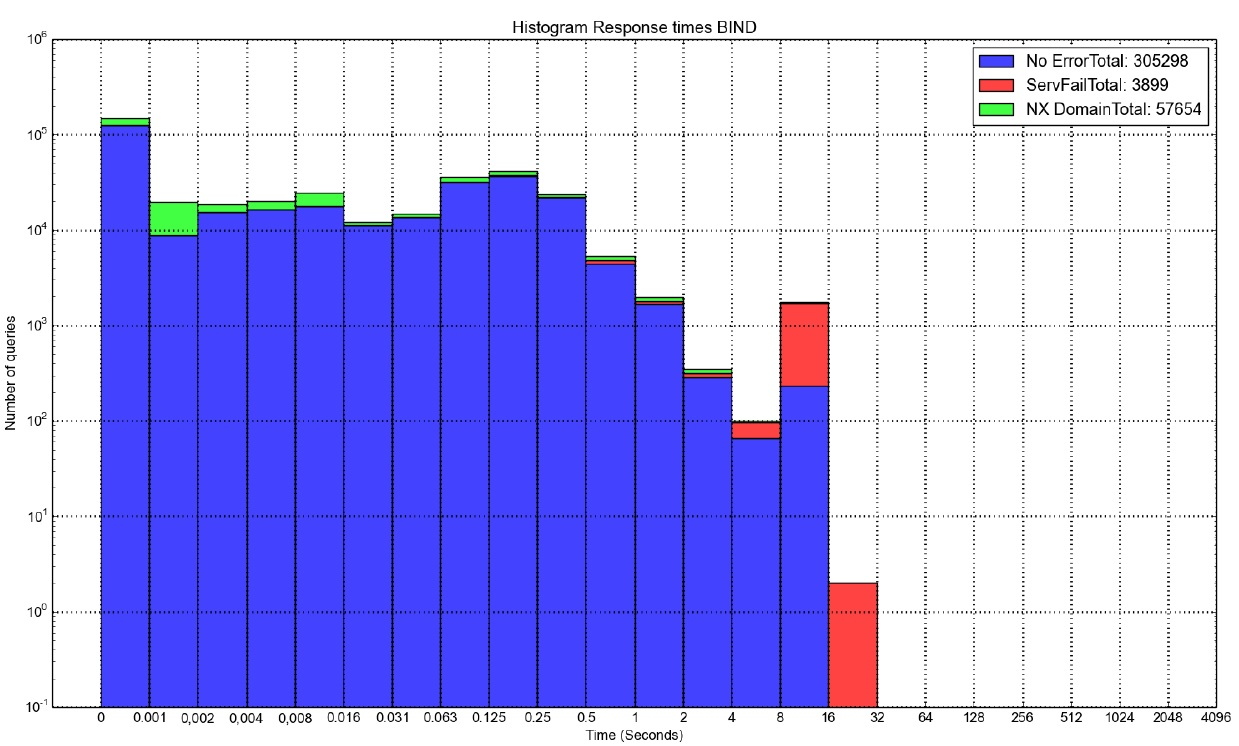
\includegraphics[width=0.8\textwidth]{figure/Measurement-BIND.jpg}
    \caption{\em The processing time in BIND \cite{DNS_resolver_performance_measurements} \label{fig:Measurement_BIND}}
\end{figure}


\begin{figure}[hbt!]  
    \centering
    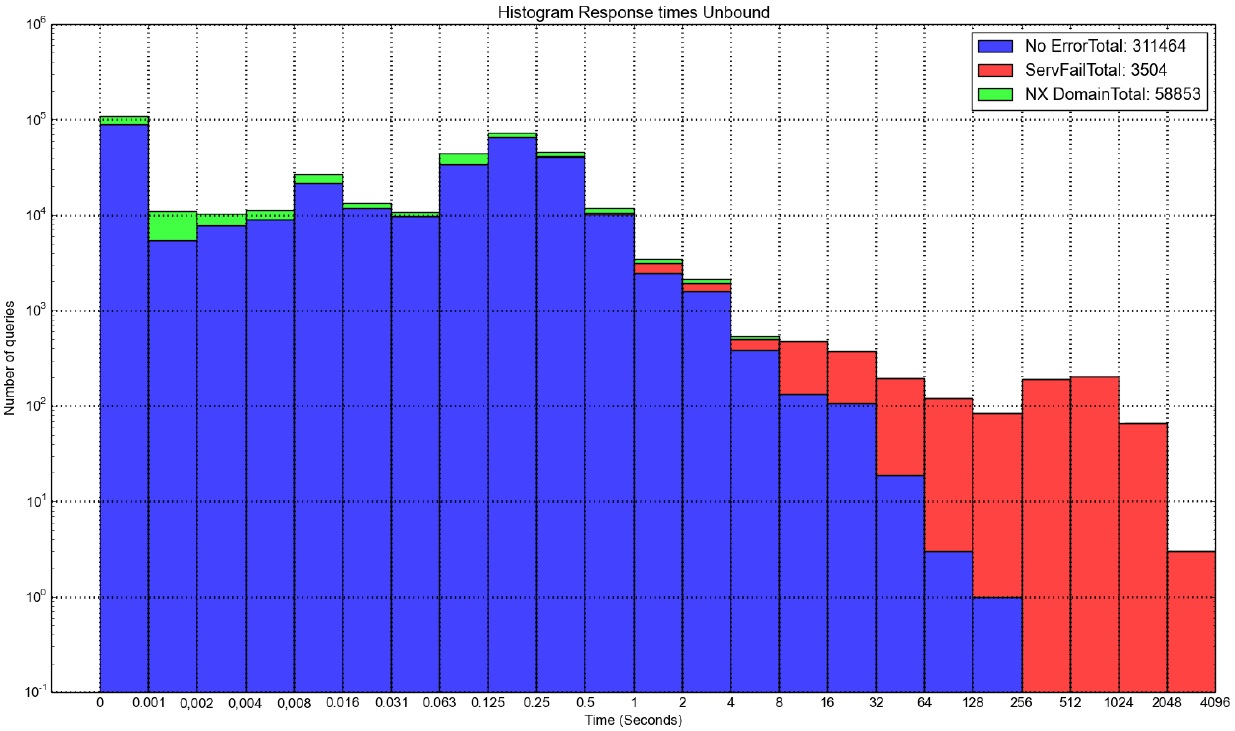
\includegraphics[width=0.8\textwidth]{figure/Measurement-Unbound.jpg}
    \caption{\em The processing time in Unbound \cite{DNS_resolver_performance_measurements} \label{fig:Measurement_Unbound}}
\end{figure}


Fig.~\ref{fig:Measurement_BIND}, Fig.~\ref{fig:Measurement_Unbound} and Fig.~\ref{fig:Measurements_PowerDNS} show the details of the time of processing queries in BIND, Unbound and PowerDNS. The working types in BIND and PowerDNS are similar, both of them have the time limit, thus in case the processing time reaches the time limit, then the query will be failed. In contrast, Unbound has a different working type, it allows the system to have a long time to wait for the answer after the process. Hamza Boulakhrif called those different working types as "Failed response over a late response" and "An answer is better than no answer". PowerDNS adopts "Failed response over a late response" and Unbound adopts "An answer is better than no answer", as for BIND, it is between PowerDNS and Unbound \cite{DNS_resolver_performance_measurements}.
\\

In conclusion, in choosing DNS resolver software, because BIND, Unbound, PowerDNS have similar performances, therefore the point of the decision is allowing a long time to wait for the answer or not. If yes, the operator should choose Unbound. Otherwise, he should choose BIND or PowerDNS.
\\

However, the report was written in 2015, which was 5 years ago, the situation may be different now.
\\

\section{Comparison of operating system}

In choosing a operation system for testing, there are many operation systems could be used to install DNS servers, such as Windows server, BSD, Linux Red Hat, Linux Ubuntu, Linux CentOS. Many developers prefer using Unix-like rather than Windows server base on the concern about stability and cost, therefore the researcher excluded Windows server.
\\

On the other hand, even though FreeBSB is a good choice for building servers, but the information of BSD is less than Linux, which means Linux is more popular, thus the researcher decided to use Linux.
\\

However, there are many members in the Linux family, including Fedora,Red Hat Linux, CentOS, Ubuntu, Debian \cite{Linux_distributions}. CentOS is chosen here, because it is free, and the structure is the offshoot of Red Hat enterprise, hence it is very stable. 
\\

\section{Installing a DOH server for TRR}

After the discussion about the performance, in order to understand the situation of the setting and usability among BIND, Unbound and PowerDNS, the researcher tried to install those 3 DNS software on a server and test them.
\\

Due to the effect of COVID-19, students were not allowed to go inside the laboratory, hence this study has to be finished at home, therefore the equipment was limited, only 4 personal devices were available to the researcher, which were a personal desktop computer, 2 android phones and a IPad. The operating system on the personal desktop computer is Windows 10. Thus, there was no spare computer to install Linux, the researcher had to use a virtual machine to install Linux on the personal computer. The software for running virtual machine was VMware Workstation Player.
\\

After installing the operation system, then installed BIND, Unbound and PowerDNS, and set the configuration files of those DNS servers, to make sure those DNS servers were in the same network zone with other testing devices.
\\

Next, used Internet Information Services(IIS) to create a simple website on the personal computer, and gave fixed local IP addresses to all devices and the virtual machine, then both the DNS server and website had the IP addresses. In the DNS server(BIND, Unbound and PowerDNS), set a domain name to the simple website to match its IP address. The simple website was the testing website.
\\

Finally, used the testing devices(Android phone and IPad) to type the domain name of the testing website on browsers(Google Chrome and Safari). If the testing website could be displayed on testing devices, then the DNS server functioned well. \\

Above steps were the testing method for the study. The testing environment is shown in TABLE ~\ref{tab:Testing_environment}.

\begin{table}[hbt!]
    \centering
    \begin{tabular}{|c|c|}
        \hline
         Platform & VMware Workstation 15.5.6 Player \\    
        \hline
         Operating system & CentOS 8.2.2004 \\
        \hline
         Internet connection & Bridge mode \\
        \hline
         Testing devices & Desktop, IPad, Android phone\\
        \hline
    \end{tabular}
    \caption{The testing environment}
    \label{tab:Testing_environment}
\end{table}

Next, the following discussion is about configuration. The configuration of BIND is using C language to be the format of the configuration file. Therefore, in case the maintenance personnel does not have programming background, then it needs time to understand the syntax of C language.
\\

About Unbound, the format of configuration file is very simple, it does not belong to any kind of computer languages. The setting is just listed line by line.
\\

PowerDNS adopts relational database, thus the configuration of PowerDNS has 2 parts, the first part is the normal configuration file, it decides the setting for the database. The second part is in the database, the contain is including domains and records.
\\

The installation of PowerDNS is more complex than Unbound and BIND, because it uses the rational database. However, it is a double-edged sword, it is not friendly for normal users during the installation, but after installation, PowerDNS provides the website to display the information of DNS server, and the website is also the interface for the setting, hence the maintenance is easier than BIND and Unbound.
\\

The comparison among BIND, Unbound, PowerDNS is shown in Table ~\ref{tab:BIND_unbound_powerDNS}.

\begin{table}[hbt!]
    \centering
    \begin{tabular}{|c|c|c|c|}
        \hline
         & BIND & Unbound & PowerDNS \\    
        \hline
         Version &  &  & \\
        \hline
         Query time limit & Short & Long & Short \\
        \hline
         Performance & Similar & Similar & Similar \\
        \hline
         Configuration & C language & Line by line  & RDBMS \\
        \hline
         Log style & Log file & Log file & MySQL \\
        \hline
         Installation difficulty & Easy & Easy & Difficult \\
        \hline
         Maintenance difficulty & Normal & Normal & Easy \\
        \hline
    \end{tabular}
    \caption{The comparison among BIND, Unbound, PowerDNS}
    \label{tab:BIND_unbound_powerDNS}
\end{table}

\section{The simulation of the internet traffic in national scale}

In previous description,  a DNS server is possible to suffer 4,494 transactions per second, therefore it is necessary to simulate this situation to the DNS server which is built by the researcher.

The researcher used Python to make a simple application, the application can send a huge number of queries to the DNS server, and the number can be changed by the researcher.

\begin{table}[hbt!]
    \centering
    \begin{tabular}{|c|c|}
        \hline
         Language & Python 3.7 \\    
        \hline
         Library &  DNS.resolver \\
        \hline
         DNS software & BIND \\
        \hline
         CPU in the server & Intel Core i7-7700(3.60GHz, 4 cores)\\
        \hline
         Memory in the server & 8G \\
        \hline
         Operating system & CentOS 8.2 in virtual machine \\
        \hline
         First testing & 100 queries for 1 domain name \\
        \hline
         Second testing & 5000 queries for 1 domain name \\
        \hline
         Third testing & 10000 queries for 1 domain name \\
        \hline
         Forth testing & 100 queries for different domain names \\ 
        \hline
         Fifth testing & 5000 queries for different domain names \\ 
        \hline
         Sixth testing & 10000 queries for different domain names \\ 
        \hline
    \end{tabular}
    \caption{The description of the application for testing massive queries}
    \label{tab:Queries_application}
\end{table}
